\section{Komponenten eines Arbeitsplatzcomputers unterscheiden}
\subsection{Zentraleinheit, Mainboard und Betriebssystem unterscheiden}
    TODO

\subsection{Hauptplatine, Mainboard und die Komponenten unterscheiden}
    \begin{figure}[ht]
        \centering
        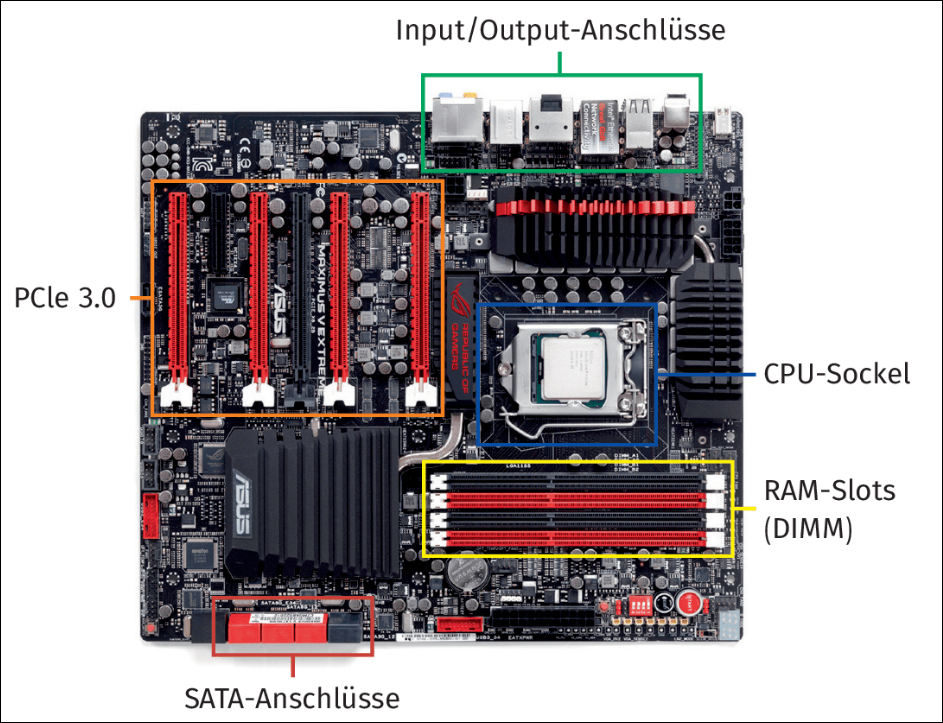
\includegraphics[width=0.7\textwidth]{./images/2.4.2_mainboard.png}
        \caption{Mainboard}\label{fig:Mainboard}
    \end{figure}
    
    \begin{subindent}
        \begin{itemize}[leftmargin=2.5cm, topsep=0.2em, itemsep=0.1em, parsep=0.3em]
            \item \textbf{Mainboard:} \\
                  auch Motherboard oder Systemplatine, Hauptplatine, auf der alle Komponenten angebracht sind
            \item \textbf{BIOS:} \\
                  zuständig für Startvorgang, enthält in \textbf{EPROM} ein Basisbetriebssystem
            \item \textbf{Chipsatz:} \\
                  zuständig für Kommunikation der Komponenten untereinander
            \item \textbf{Sockel:} \\
                  physikalische Verbindung von Mainboard und Prozessor
            \item \textbf{Peripherie-Anschlüsse, (PCIe-)Steckplätze:} \\
                  I/O-Peripherie für externe Hardware (z.B. Maus/Tastatur) \\
                  Steckplätze auf Mainboard für interne Hardware (z.B. RAM, GPU oder SATA/M.2)
            \item \textbf{Netzteil:} \\
                  Stromversorgung aller Komponenten
        \end{itemize}
    \end{subindent}
    
    \begin{figure}[ht]
        \centering
        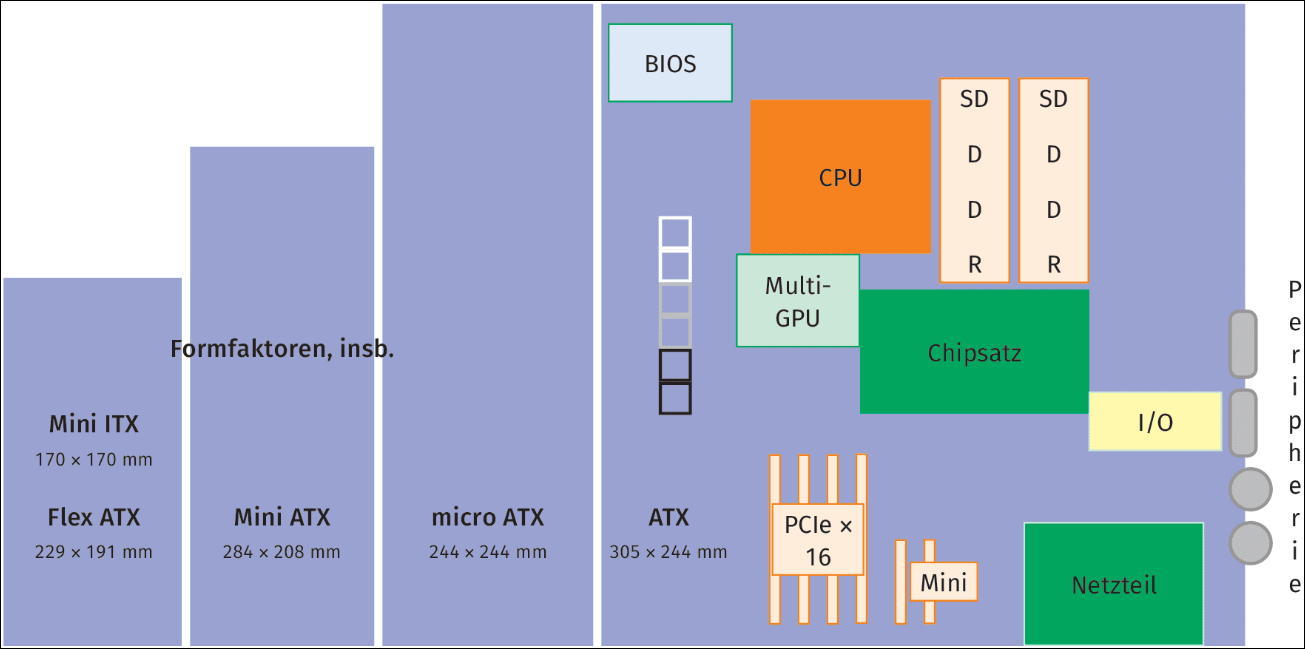
\includegraphics[width=0.7\textwidth]{./images/2.4.2_formfaktoren.png}
        \caption{Formfaktoren}\label{fig:Formfaktoren}
    \end{figure}

\newpage
\subsection{Prozessoren genauer beschreiben}
    TODO

\subsection{Arbeistspeicher (RAM-Speicher) erläutern}
    \begin{subindent}
        RAM-Speicher (Random Access Memory) ist ein flüchtiger Arbeitsspeicher, über den die CPU auf Daten zugreift, wenn mehrere Programme parallel benutzt werden. Da RAM flüchtig ist werden die Daten beim Herunterfahren des PCs gelöscht. \\
        RAM-Formate:
        \begin{itemize}[leftmargin=2.5cm,, itemsep=0.1em, parsep=0.3em]
            \item DIMM\@: Dual In Line Memory Module, wird in Desktops und Servern verwendet
            \item SO-DIMM\@: Small Outline DIMM, wird in Laptops verwendet
        \end{itemize}
        Neben dem Arbeitsspeicher gibt es noch den (im Vergleich zur RAM) schnellen Cache-Speicher. \\
        Cache-Levels:
        \begin{itemize}[leftmargin=2.5cm, itemsep=0.1em, parsep=0.3em]
            \item L1-Cache: Geschwindigkeit ähnlich zu Prozessor, für häufig verwendete Befehle und Daten
            \item L2-Cache: größer und langsamer als L1, aber schneller als RAM
            \item L3-Cache: Datenabgleich Caches und Cores
        \end{itemize}
        Die Geschwindigkeiten werden in Megatransfers per Second (MT/s) angegeben.
    \end{subindent}

    \begin{figure}[ht]
        \centering
        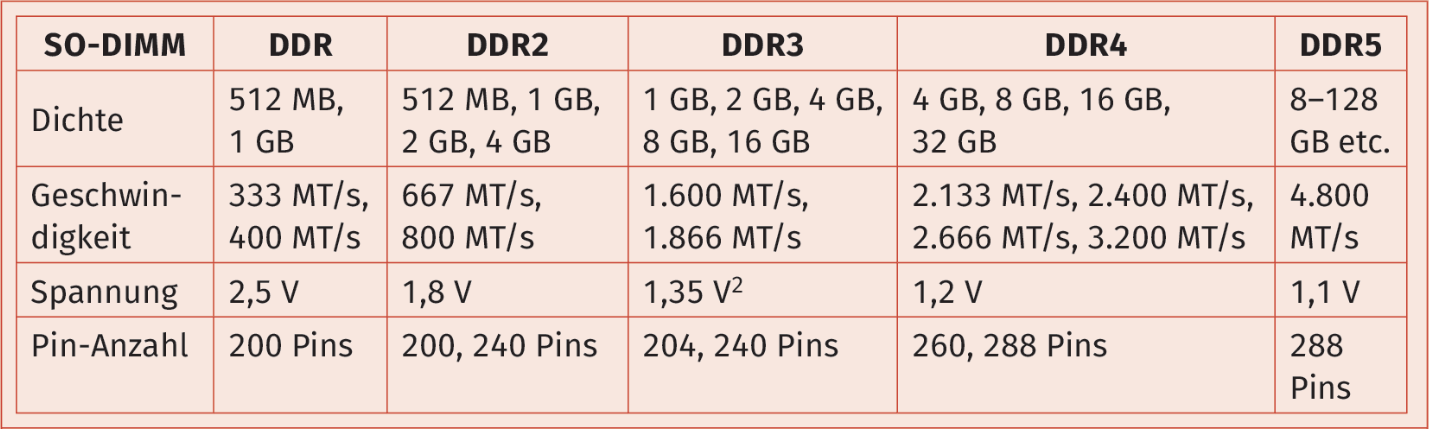
\includegraphics[width=0.7\textwidth]{./images/2.4.4_ramspeeds.png}
        \caption{RAM-Geschwindigkeiten}\label{fig:RAM-Geschwindigkeiten}
    \end{figure}

    \begin{tcolorbox}[width=15cm, center, title=RAM Begriffe, coltitle=white, colframe=orange, colback=white!60!orange]
        \begin{itemize}[itemsep=0.1em, parsep=0.3em]
            \item RAM\@: Random Access Memory
            \item JEDEC\@: \\ Joint Electronic Device Engineering Council \\ Organisation legt Spezifikationen für elektrische und zeitliche Parameter der Speichercontroller und -chips fest
            \item Formfaktoren: \\ UDIMM (Unbuffered DIMM): häufigstes Format in Desktops \\ SO-DIMM\@: kleiner und physikalisch kürzer als UDIMMS
            \item DRAM\@: Dynamic Random Access Memory \\ Jedes Datenbit wird auf seperatem Kondensatoren gespeichert
            \item SDRAM\@: Synchronous Dynamic Random Access Memory \\ getaktetes DRAM, Daten werden synchron zum Speicher-Bus übertragen
            \item DDR-RAM\@: Double Data Rate RAM \\ überträgt Daten doppelt so schnell wie SDRAM\@; neueste Generation ist DDR5 (Gens untereinander nicht kompatibel)
            \item DDR-SDRAM\@: Weiterentwicklung der SDRAM-Technologie
            \item SSD-RAM\@: Solid State RAM \\ flash-based Speicher, SSD-Speicher wird als zusätzliche RAM benutzt, die Daten darauf bleiben beim Herunterfahren erhalten
            \item QLC\@: Quad-Level-Cells \\ neueste Tech der Flash-Speicherarchitektur, speichert vier Datenbits in jeder Datenzelle
            \item FSB\@: Frontsidebus \\ Hauptpfad für Daten im Computer, verbindet CPU, DRAM, GPU und Chipsatz
            \item Latenz\@: Zeit, die Speicher benötigt, um auf Befehl zu reagieren
            \item ECC\@: Error Correcting Code \\ teures `fully buffered, registered ECC RAM', das hilft Speicherfehler zu minimieren oder selbst zu korrigieren 
        \end{itemize}
    \end{tcolorbox}

\subsection{Schnittstellen und Anschlüsse am Mainboard erläutern}
    \begin{figure}[ht]
        \centering
        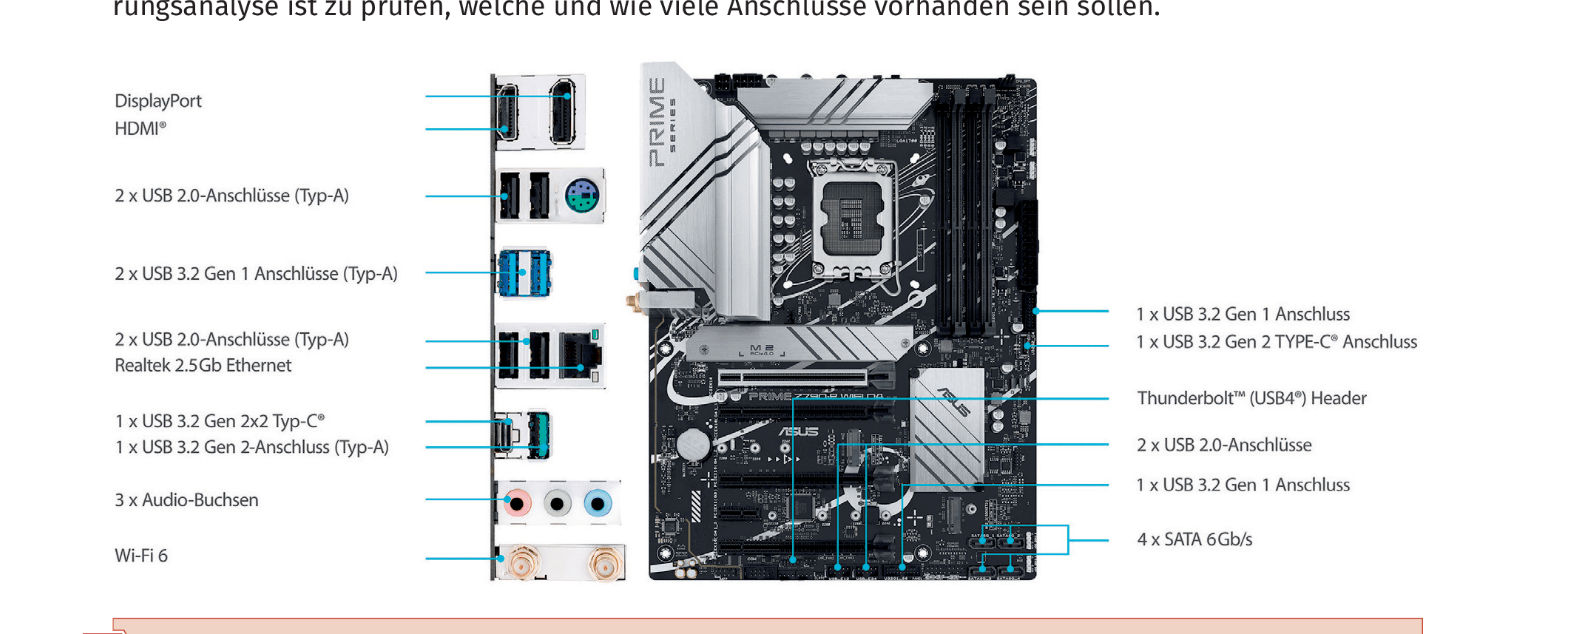
\includegraphics[width=0.7\textwidth]{./images/2.4.5_anschluesse.png}
        \caption{Mainboard Anschlüsse}\label{fig:Mainboard Anschlüsse}
    \end{figure}

    \begin{tcolorbox}[width=15cm, center, title=Anschlüsse am Mainboard, coltitle=white, colframe=orange, colback=white!60!orange]
        \begin{itemize}[itemsep=0.1em, parsep=0.3em]
            \item Sockel\@: Ort in dem der Prozessor platziert wird
            \item RAM-Steckplätze
            \item PCI(e)-Steckplätze\@: Peripheral Component Interconnect Express (PCIe) \\ Anschluss von Zusatzkarten, verfügbare Steckplätze sind abhängig vom Motherboard
            \item SATA-Anschlüsse\@: Verbindung von Festplatten und Laufwerken \\ Blaue SATA-Buchsen: 6 GBit/s, Abwärtskompatibel \\ Schwarze/Rote SATA-Buchsen: Herstellerabhängige Bedeutung
            \item USB-Schnittstellen\@: Schnittstellen für USB-Ports
            \item M.2-Port\@: Anschluss für SDD
            \item Lüfteranschluss
            \item Stromanschluss
            \item Monitoranschlüsse
            \item USB-Anschlüsse
            \item P/S2-Port\@: Anschluss für ältere Mäuse und Tastaturen
            \item LAN
            \item Klinkenanschlüsse\@: Tonübertragung
        \end{itemize}
    \end{tcolorbox}

    \begin{figure}[ht]
        \centering
        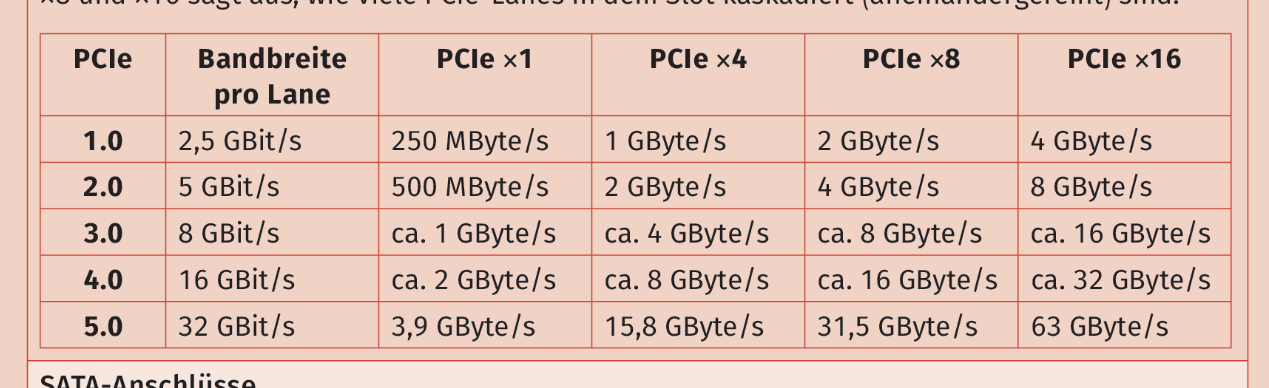
\includegraphics[width=0.7\textwidth]{./images/2.4.5_pciespeeds.png}
        \caption{PCIe Geschwindigkeiten}\label{fig:PCIe Geschwindigkeiten}
    \end{figure}

    \begin{figure}[ht]
        \centering
        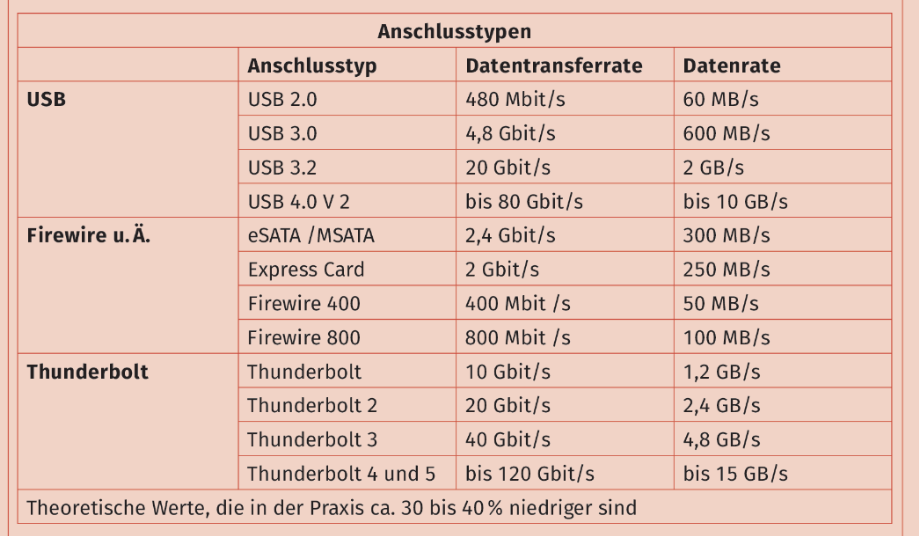
\includegraphics[width=0.7\textwidth]{./images/2.4.5_usbspeed.png}
        \caption{USB Geschwindigkeiten}\label{fig:USB Geschwindigkeiten}
    \end{figure}

\newpage
\subsection{Netzteile beschreiben und unterscheiden}
    TODO
\subsection{Festplatten unterscheiden und erläutern}
    TODO
\subsection{Tastaturen unterscheiden und präsentieren}
    TODO
\subsection{Monitore vergleichen und präsentieren}
    TODO
\subsection{Leistungsmerkmale für Drucker und Zusatzanforderungen erläutern}
    TODO (aktueller Fortschrittsstand)
\subsection{Scanner beschreiben und für Arbeitsplatz auswählen}
    TODO
\subsection{IT-Zubehör für die Barrierefreiheit und im Aftersales unterscheiden}
    TODO
\subsection{Unternehmenssoftware anbieten und vergleichen}
    TODO
\subsection{Marktgängige IT-Systeme und Lösungen anbieten}
    TODO
\subsection*{Reflexion Kapitel 2.4}
\addcontentsline{toc}{subsection}{Reflexion Kapitel 2.4}
    %TODO REFLEXION
    \begin{refindent}
        TODO
    \end{refindent}